\documentclass{article} % for short documents
%\documentclass{report} % for longer documents

\usepackage{minted}

%% Defining the language for the document
\usepackage[english]{babel}
\usepackage[english]{isodate}

\usepackage{imta_core}
\usepackage{imta_extra}
\usepackage{epigraph}
\usepackage{graphicx}
\usepackage{wrapfig}
\usepackage{alertmessage}
\usepackage{hyperref}
\usepackage{xcolor}


%% Addtionnal packages can be loaded here
% \usepackage{biblatex} % for a complete and flexible bibliography


\cleanlookdateon % formats date according to the loaded language from now on

%% General informations
\author{\\ Alexandre ALLANI \\
Adrien CLOTTEAU \\
François GUIBOURT \\
Vincent HIAULT \\
Yann BOUENAN}
%\imtaAuthorShort{<author's initials>}
%\imtaSuperviser{<superviser>}
\date{\noexpand\today} % automatically print today's date, can be redefined using \date{<date>}
\title{Projet Aide à la décision}
\subtitle{Algorithme génétique}
%\imtaVersion{<version>}

%Add extra other companies' logo
%If needed, options can be passed to the underlying \includegraphics by calling \imtaAddPartnerLogo[<options>]{<path>}
%\imtaAddPartnerLogo{<logo_path>}


\imtaSetIMTStyle % Sets font and headers/footers according to the IMT Atlantue style guidelines


%%%%%%%%%%%%%%%%%%%%%%%%%%%%%%% 
%%%%%%%%%% BEGINNING %%%%%%%%%% 
\begin{document}

% front cover
\imtaMaketitlepage
\tableofcontents
\newpage
\section{Introduction}
Le problème qui va être traité concerne l'optimisation de la location de hub au sein d'un réseau. Nous avons à disposition une liste de lieu devant être connectés les uns aux autres par un réseau. Certains lieux (nœuds au sein d'un graphe), peuvent être des hubs, c'est à dire connectés à plusieurs autres lieux. Tandis que d'autres lieux vont être des spokes, c'est à dire qu'ils ne communiquent qu'avec un seul hub. Pour résumer, un Hub est connecté à des hubs/spoke et un spoke est connecté au maximum à un hub (Single allocaiton hub problem). Il est supposé par la suite, que les lieux sont fixes et que chaque lieux doit être connecté au réseau.\\

Le problème va être d'optimiser les contraintes qui vont régir le réseau. Pour chaque hub nous avons les contraintes suivantes :
\begin{itemize}
	\item Coût fixe (propre au noeud)
	\item Coût Variable (dépendant du flux de marchandise passant par le noeud). 
	\item Le transfert de flux entre deux hub est soumis à une réduction de coût
	\item Chaque hub a une capacité de marchandise limitée
\end{itemize}

Il est possible de résoudre de manière optimale ce problème sur un nombre limité de ville en utilisant les méthodes de résolutions linéaires (avec GLPK par exemple). Cependant ici nous nous concentrons sur un problème rassemblant plus de 30 locations différentes. Nous avons donc choisi d'utiliser un algorithme génétique pour trouver une solution optimale à ce problème.\\


Le but de ce rapport est de décrire le design de notre algorithme génétique, ainsi que son implémentation. Nous présenterons ensuite les résultats que nous avons eu, ainsi que l'influence des différents paramètres sur la résolution du problème.

\alertinfo{Vous pouvez retrouver le code sur le lien suivant.La manière de lancer l'algorithme y est aussi expliqué. \url{https://github.com/Syndorik/Genetic-Algorithm}. 
}
\newpage
\section{Design de l'algorithme génétique}
Dans cette partie nous allons voir comment a été designé l'algorithme génétique pour résoudre le problème de location de hub.

\subsection{Représentation des solutions}
~\\
\begin{wrapfigure}[12]{L}{100mm}
	\centering
	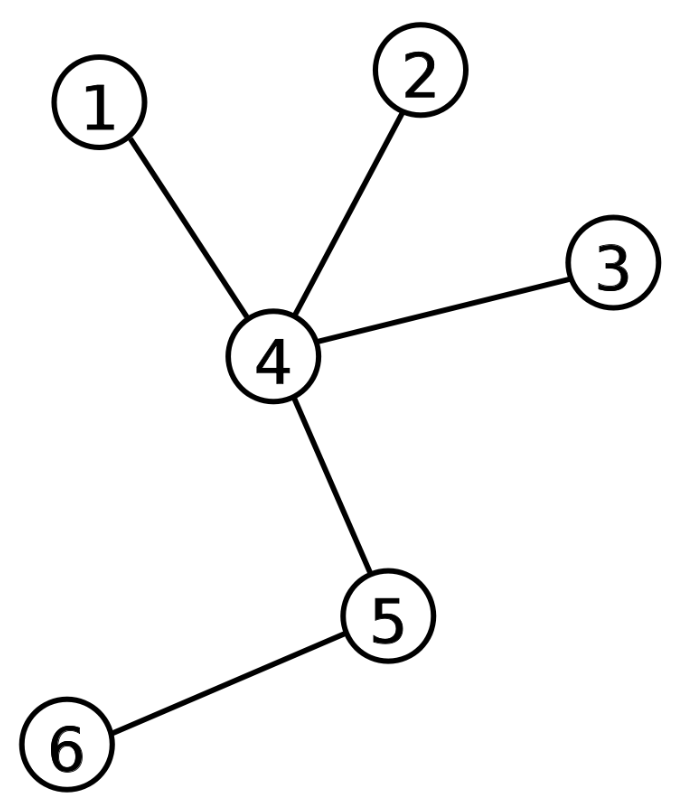
\includegraphics[keepaspectratio = true,scale=0.2]{prufer.png}
	\caption{Graphe obtenu à partir du code Prüfer : [4,4,4,5]}
\end{wrapfigure}
Avant de travailler sur l'algorithme génétique en lui même il est important de trouver une représentation conforme des solutions. Le but est de trouver une structure permettant de décrire une solution à ce problème. En particulier, il faut qu'elle respecte la contrainte de \textit{single allocation}, qu'il soit possible de distinguer les hubs des spokes et qu'il n'y ait pas de spokes non connectés au réseau.\\

Pour cela nous avons choisi de travailler avec un codage de Prüfer. Le code de Prüfer une fois décodé nous donne accès à un graphe qui représentera la solution proposée. De plus les nœuds contenus dans le code de Prüfer correspondent aux hubs (car cela implique la connexion avec au moins 2 nœuds), et, inversement, ceux qui ne sont pas dedans sont les spokes.\\~\\~\\
L'exemple de la \textbf{Figure 1} montre bien que les nœuds $4$ et $5$, présents dans le code de Prüfer,  sont effectivement des hubs , tandis que les noeuds $1$, $2$, $3$ et $6$ sont des spokes. Cette représentation convient donc parfaitement comme base de l'algorithme génétique.

\subparagraph{Fitness function\\}
La fitness function est ce que l'on cherche à optimiser dans la création du réseau. Elle est accessible via ce \href{http://formations.telecom-bretagne.eu/or/courses/2018-2019-ISA/03/03.html}{\underline{\textbf{\textcolor[rgb]{0,0,1}{lien}}}}. Cette fonction résume simplement les différents coûts à minimiser pour l'ensemble du réseau, les coûts fixes pour les hubs et les coûts variables dépendant du flux traversant le réseau.

\subsection{Opérateur de Crossover}
Afin de créer une nouvelle génération, nous devons établir un moyen de mélanger les différents individus. L'idéal serait que cette opération de \textit{crossover} ne donne pas de solution irréalisable. Dans notre cas, la capacité de chaque hub doit être respectée, sinon le réseau ne peut pas être crée.\\ 

\begin{wrapfigure}[9]{L}{60mm}
	\centering
	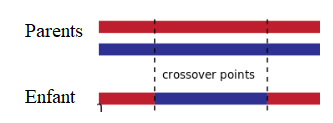
\includegraphics[keepaspectratio = true,scale=0.8]{kpoint.png}
	\caption{Two-point crossover}
\end{wrapfigure}
Il était difficile de trouver un opérateur ne retournant pas de solution irréalisable. Nous avons choisi l'opérateur \textit{k-point crossover}. Le principe est de diviser le code de Prüfer des deux parents en k points différents (k étant fixé en tant que paramètre), et ensuite de réaliser un crossover normal, c'est à dire échanger les différentes parties du code de Prüfer. La \textbf{Figure 2} illustre ce procédé pour un $k=2$.\\
Afin de pallier au problème possible de non conformité des solutions, nous avons choisi d'affecter une valeur très grande à la fitness function. Ainsi, lors de l'étape de la sélection \textbf{Section 2.3}, ces solutions auront peu de chance d'être sélectionnées. De plus, ceci va rajouter un paramètre à l'algorithme génétique en plus de ceux déjà existant (nombre d'individus dans la population, nombre de génération maximale, probabilité de mutation).

\subsection{Opérateur de Sélection}
Le but de cet opérateur est de sélectionner les solutions parmi une population d'individus qui vont être les parents utilisés dans l'opérateur de \textit{crossover}. Ici nous utilisons un \textit{k-way torunament}. Le principe est de choisir k individus dans la population de base. Ensuite un tournois est fait entre ces k individus, et celui qui a la meilleure fitness est choisi (ie, l'individu qui a la plus faible fitness parmi les k individus).\\
Dans l'algorithme, cela permet de choisir les deux parents auxquels vont être appliqué l'opérateur de crossover. Ce processus (Sélection par tournois + crossover) répété assez de fois permet de créer la population descendante. Cependant, il est à noter que s'il y a élitisme, le meilleur individu de la population initial sera conservé dans la population descendante.\\
Cet opérateur permet de privilégier les individus ayant une bonne fitness (vu qu'ils vont gagner les tournois s'ils sont sélectionnés) tout en gardant des individus moins bons permettant de faire un peu plus d'exploration (et donc de retourner moins souvent un minimum local). Ceci rajoute donc un autre paramètre à notre algorithme : le nombre k d'individus à choisir pour un tournois.\\


\subsection{Opérateur de mutation}
Cet opérateur permet d'avoir plus de variété au sein de la population et d'effectuer des opérations impossibles par crossover. Ici nous avons créé plusieurs opérateurs de mutation différents que nous avons testé.
\alertinfo{Les fonctions de mutations sont disponnibles dans le fichier nommé GA.py disponnible sur \url{https://github.com/Syndorik/Genetic-Algorithm/blob/master/lib/GA.py}. 
}
Dans les paragraphes qui suivent nous explicitons chaque opérateur de mutation créé, et si nous l'avons finalement gardé. Nous partons du principe que la condition de probabilité est remplie dans chacun des cas. Les mutations effectuées se basent soit sur la fonction \textbf{swap} soit la fonction \textbf{swap\_2opt}

\subparagraph{Opérateur swap\\}
A partir d'un code de Prüfer , deux indices sélectionnés au préalable sont échangés. Exemple pour un code de Prüfer $ = [4,4,5,6,2,2,6,8]$ et les indices $2$ et $5$ :
\begin{figure}[!h]
	\centering
	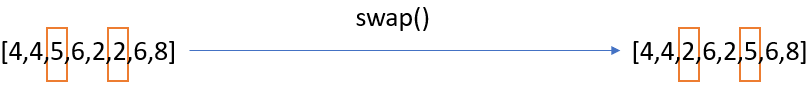
\includegraphics[keepaspectratio = true,scale=0.8]{mutate.png}
	\caption{swap operator}
\end{figure}

\subparagraph{Opérateur swap\_2opt\\}
A partir d'un code de Prüfer, et deux indices sélectionnés au préalables, une inversion de la route créé par l'ensemble des éléments compris entre les indices (indices exclus) est réalisé. Exemple pour un code de Prüfer $ = [1,5,4,3,2,6]$ et les indices $0$ et $5$ :
\begin{figure}[!h]
	\centering
	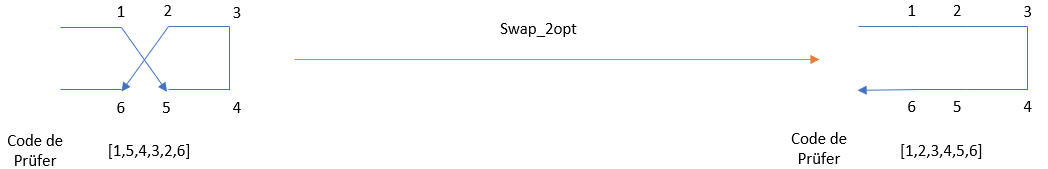
\includegraphics[keepaspectratio = true,scale=0.8]{2opt.png}
	\caption{swap\_2opt operator}
\end{figure}
\newpage
\subsubsection{Fonction : mutate}
Cet opérateur est l'opérateur le plus basique. Il se base sur la fonction swap.
Le principe est simple, deux indices du code de Prüfer de l'individu sont tirés, la fonction swap est appliquée et l'individu modifié est retourné.\\
Cette fonction est très rapide à exécuter mais ne donne pas des résultats assez satisfaisant. 

\subsubsection{Fonction : mutate\_swap}
Cet opérateur ce base sur la fonction swap. Ici, au lieu de faire des permutations aléatoires, nous allons tester les permutations possibles une par une jusqu'à obtenir une permutation donnant un individu dont la fitness est meilleure que celle de l'individu original. Une fois obtenue,  l'algorithme ne cherche plus de meilleurs permutation et l'individu modifié est retourné. Dans le cas où aucunes permutations ne donne un meilleur individu, l'individu originel est retourné.\\
Cette fonction est assez bonne en terme d'exploitation. Le local search appliqué permet d'avoir des individus qui sont toujours meilleurs (ou du moins tout aussi bien) que l'individu original. Cependant, le temps d'exécution est assez long, et il est assez fréquent de tomber dans un minimum local et ne plus pouvoir en sortir.\\
Cela s'explique par le fait que les individus une fois muté ne laissent plus assez de place pour l'exploration car il y a moins d'individus ayant de moins bonnes fitness.

\subsubsection{Fonction : mutate\_swap\_nerfed \\}
Ici,le même principe de fonctionnement de la fonction \textit{mutate\_swap} est utilisé. Cependant cette fois-ci, il n'y a pas de permutations sur l'ensemble des permutations, mais uniquement sur un échantillon d'indices pris aléatoirement (correspondant à 1/3 des indices du code de Prüfer). De plus si aucune mutation améliore la fitness, ce n'est pas l'individu original qui est renvoyé, mais l'individu ayant eu la meilleure fitness parmi tout les individus créés.


Cette alternative se retrouve être la meilleure. Le temps d'exécution est assez court et les résultats convaincants. Cela s'explique par le fait que le local search est bien plus limité que pour la fonction \textit{mutate\_swap} au vu des modifications apportées. Il y a alors un bon compromis entre \textbf{exploration et exploitation}

\subsubsection{Fonction : mutate\_2opt\\}
De même, le principe de fonctionnement de \textit{mutate\_swap} est repris, la fonction de permutation utilisée n'est pas \textit{swap} mais \textit{2opt}.\\
Les résultats obtenus étaient assez décevant et le temps d'exécution très long.

\subsection{Critères d'arrêts}
Deux critères ont été retenus pour arrêter l'algorithme génétique :
\begin{itemize}
	\item \textbf{Nombre d'itération} : ou nombre de génération. Après un certain nombre d'itération, l'algorithme s'arrête. Ce critère permet de ne pas rester coincé dans une boucle infinie. En général il n'est pas atteint car le second critère est atteint avant. Le nombre de génération est un paramètre mais pour l'ensemble des tests effectués, il a été fixé à 100. Parmi les 68 tests réalisés, il n'a jamais été atteint.
	\item \textbf{Evolution de fitness nulle} : Si au bout d'un certain nombre d'itération, la fitness n'évolue plus l'algorithme s'arrête. Ce critère d'arrêt a été fixé à 8. Ainsi, s'il n'y a plus d'amélioration au bout de 8 itérations l'algorithme est arrêté. Ce critère d'arrêt est souvent atteint. 8 générations sont laissées car il est possible de sortir du minimum local par exploration (crossover)
\end{itemize}
\newpage
\subsection{Déroulement de l'algorithme génétique}
\alertinfo{Le code correspondant à cette étape est disponnible dans le fichier App.py \url{https://github.com/Syndorik/Genetic-Algorithm/blob/master/lib/App.py}}
Nous avons désormais l'intégralité des éléments pour créer l'algorithme génétique. Dans le cas standard, les paramètres suivants sont utilisés:
\begin{itemize}
	\item Nombre de génération : 100
	\item Taille de la population : 100
	\item Probabilité de mutation : 0.4
	\item K point crossover : 3
	\item Taille du tournois : 7
	\item Élitisme : Il y en a
	\item Méthode de permutation : swap
\end{itemize}
La première génération est composé de 100 individus dont le code de Prüfer est généré aléatoirement parmi les nœuds disponibles. Ensuite, à chaque itération (qui peut aller jusqu'à un nombre maximal de 100 dans notre cas), on va appliquer le processus suivant:
\begin{itemize}
	\item Evolution :\begin{itemize}
		\item Création de la population descendante: avec l'élitisme, le meilleur individu de la population initial est inclus dans la population descendante. Par la suite, la population descendante est complétée comme expliqué \textbf{section : 2.3}
		\item La population étant créé, on applique l'opérateur de mutation. La population descendante est alors créée.
	\end{itemize}
	\item Local search : Si au bout de 3 itérations, la fitness n'évolue plus, le processus suivant est appliqué :\begin{itemize}
		\item Sélection des 5 meilleurs individus (en terme de fitness)
		\item Pour chaque individu, l'ensemble des 2 permutations possibles va être testé, et le meilleur individu est retourné.
		\item Si parmi les 5 meilleurs individus, il y a des doublons (des individus ayant le même code de Prüfer), le processus se répète jusqu'à obtenir 5 individus différents.
	\end{itemize}
	\item Critère d'arrêt: si un des critères d'arrêt est atteint, l'algorithme s'arrête et retourne le meilleurs résultat.
\end{itemize}
L'étape de Local Search est très importante dans l'algorithme, car cela permet souvent de sortir d'un minimum local en renouvelant la population. Cependant, l'appliquer sur un grand pourcentage de la population pourrait limiter les capacités d'exploration de l'algorithme. C'est pour cela que nous nous limitons à 5 individus différents.
\newpage
\section{Résultats et tests}
\alertinfo{Vous pouvez retrouver les résultats des tests dans le dossier \textbf{log}. Le script lancé pour obtenir ces résultats est disponnible dans le dossier \textbf{script}. \url{https://github.com/Syndorik/Genetic-Algorithm}. 
}
Dans cette partie nous allons montrer le meilleur résultat obtenu (paramètres inclus) ainsi que les différents tests réalisés pour tester notre algorithme.

\subsection{Meilleur Résultat}
Le meilleur résultat, sur l'ensemble des exécutions est obtenu avec les paramètres par défaut.\\
La fitness est de $1.579\times 10^8$\\
Le code de Prüfer associé est : \\\textbf{[22, 20, 0, 24, 18, 26, 19, 1, 11, 15, 17, 14, 11, 20, 11, 6, 11, 16, 17, 11, 6, 6, 11, 11, 25, 11, 11, 23]}
\begin{figure}[!h]
	\centering
	\includegraphics[keepaspectratio = true,scale=1]{thesol.png}
	\caption{Meilleure solution trouvé par l'algorithme}
\end{figure}
\subsection{Tests}
L'algorithme étant assez long à s'exécuter, il est assez difficile de faire une vraie étude statistique avec une centaine d'échantillon pour prouver les tendances que nous allons expliciter ci-dessous.\\
Ils faut donc prendre avec précaution les analyses faites ci-dessous.

\subsubsection{Test sur la taille de la population et le nombre d'individus dans un tournois }
Ce test est réalisé sur deux paramètres car lors des tests préliminaires (tests lancés lors de la création de l'algorithme), les deux éléments semblaient être étroitement liés.\\
Les tests ont été effectué avec les paramètres par défaut excepté pour les paramètres suivants :
\begin{itemize}
	\item Nombre d'individus dans la population : [50,100,150,200,250,300]
	\item Nombre d'individus dans le tournois : [3,5,7,10]
\end{itemize}
Pour chaque combinaisons possibles de paramètre l'algorithme a été lancé et les valeurs de fitness ont été enregistré ainsi que le code de Prüfer associé.\\
\begin{figure}[!h]
	\centering
	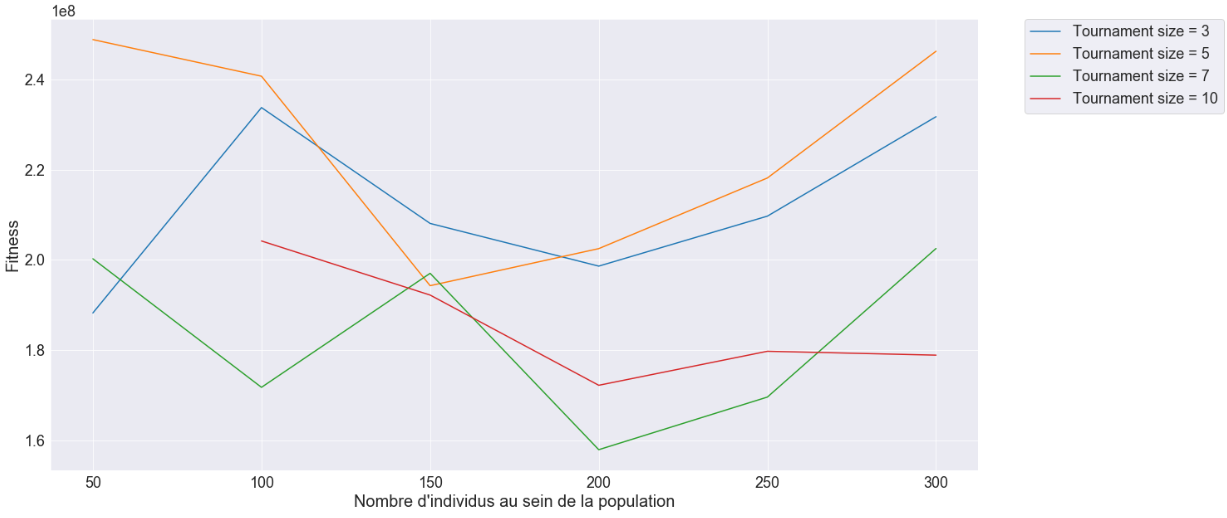
\includegraphics[keepaspectratio = true,scale=0.65]{tournAndPop.png}
	\caption{Influence des paramètres taille de la population et taille du tournois}
\end{figure}
~\\
Une certaine tendance entre les deux paramètres peut être observé: plus la population est grande, plus la taille du tournois doit être grande aussi afin d'avoir une fitness correct. Inversement, si la taille de la population est petite, il est intéressant d'avoir un petit tournois.\\
Cela s'explique par le fait qu'un tournois petit pour une grande population va être semblable à sélectionner au hasard les individus. Donc il y a très peu de bons individus qui vont être dans la population descendante. Tandis que pour un tournois grand au sein d'une petite population, le tournois va en général toujours donner les mêmes résultats (les mêmes individus). Donc il y aura très peu de diversification au sein de la population menant assez rapidement à un minimum local.\\

Pour des questions de temps d'exécution, une solution avec une population moyenne et une taille de tournois moyenne peut être privilégié. Dans les cas de nos tests, il s'avère que les meilleurs performances sont obtenus pour une taille de population égale à 200 et une taille de tournois égale à 7. Il est possible qu'avec une taille de tournois plus grande, et une population tout aussi grande les résultats soient meilleurs. Cependant nous allons rester sur les paramètres par défaut de l'algorithme (ie taille de la population = 200 et taille du tournois = 7)

\subsubsection{Test sur le k point crossover}
Le but de ce test est de voir l'influence du nombre de "coupe" dans le crossover sur la fitness finale. Les tests ont été effectué avec les paramètres par défaut excepté pour les paramètres suivants :
\begin{itemize}
	\item Le nombre de "coupe" k : [1,2,3,4]
\end{itemize}
Pour chaque combinaisons possibles de paramètre l'algorithme a été lancé et les valeurs de fitness ont été enregistré ainsi que le code de Prüfer associé.


\subsubsection{Test sur la probabilité de mutation}
Le but de ce test est de voir l'influence de la probabilité de mutation sur la fitness finale. Les tests ont été effectué avec les paramètres par défaut excepté pour le paramètre suivant :
\begin{itemize}
	\item Probabilité de mutation m : [0.1,0.3,0.4,0.6,0.8]
\end{itemize}
Le temps d'exécution étant long, nous avons lancé les tests 4 fois pour chaque probabilité de mutation. Le graphique ci-dessous est basé sur la médiane des résultats obtenus. Deux autres graphiques sont disponibles en \textbf{Annexe : 4.1}. Le premier est le même graphique mais basé sur la moyenne, le second représente la répartition des différents tests.
\begin{figure}[!h]
	\centering
	\includegraphics[keepaspectratio = true,scale=0.65]{mutationProb.png}
	\caption{Médiane des probabilités de mutations}
\end{figure}
Selon le graphique, plus la probabilité de mutation est grande, meilleur sont les résultats (que ce soit en médiane ou en moyenne). Cela paraît assez logique, car une grande partie de notre local search est effectué dans la fonction de mutation. Ainsi, lorsqu'il y a peu de mutation, il y a peu de local search, donc des solutions moins optimisés.\\
Il est cependant étonnant de voir qu'une forte probabilité de mutation entraîne de meilleurs performances qu'une probabilité moyenne car l'exploitation est privilégié à l'exploration. Donc le risque d'être dans un minimum local est plus grand.\\

\subsubsection{Test sur la méthode}
Le but de ce test est de voir quelle méthode de permutation est la meilleure pour notre problème. Les tests ont été effectué avec les paramètres par défaut excepté pour lz paramètre suivant :
\begin{itemize}
	\item méthode : ["swap","2opt"]
\end{itemize}
Pour chaque combinaisons possibles de paramètre l'algorithme a été lancé et les valeurs de fitness ont été enregistré ainsi que le code de Prüfer associé.
\newpage
\section{Annexe}
\subsection{Graphique sur les mutations}
\subsubsection{Répartitions selon les tests}
\begin{figure}[!h]
	\centering
	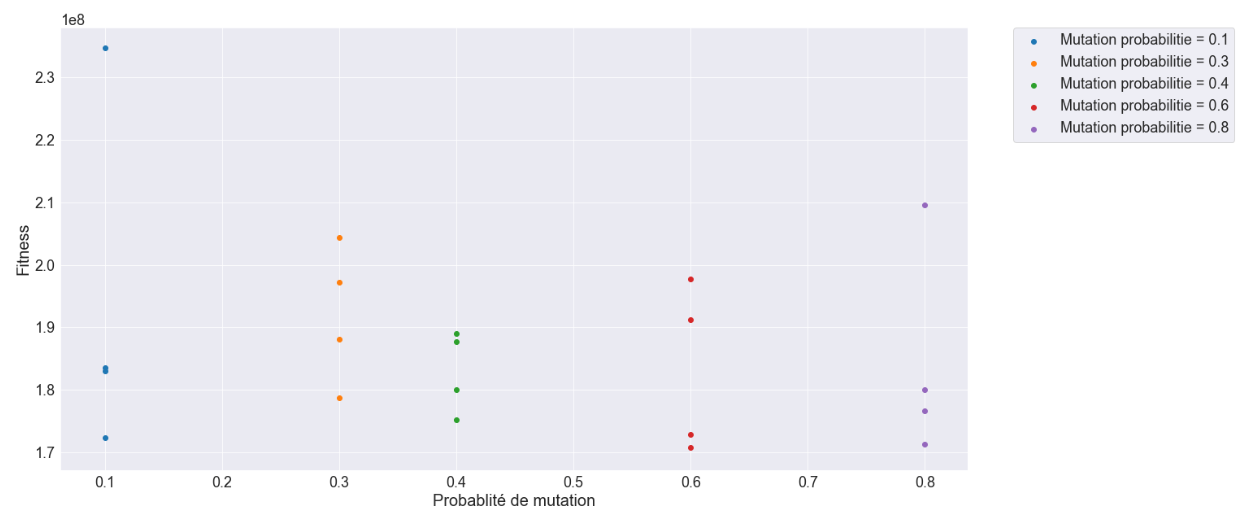
\includegraphics[keepaspectratio = true,scale=0.65]{mutation_test.png}
\end{figure}
\subsubsection{Moyenne de la fitness en fonction de la probabilité de mutation}
\begin{figure}[!h]
	\centering
	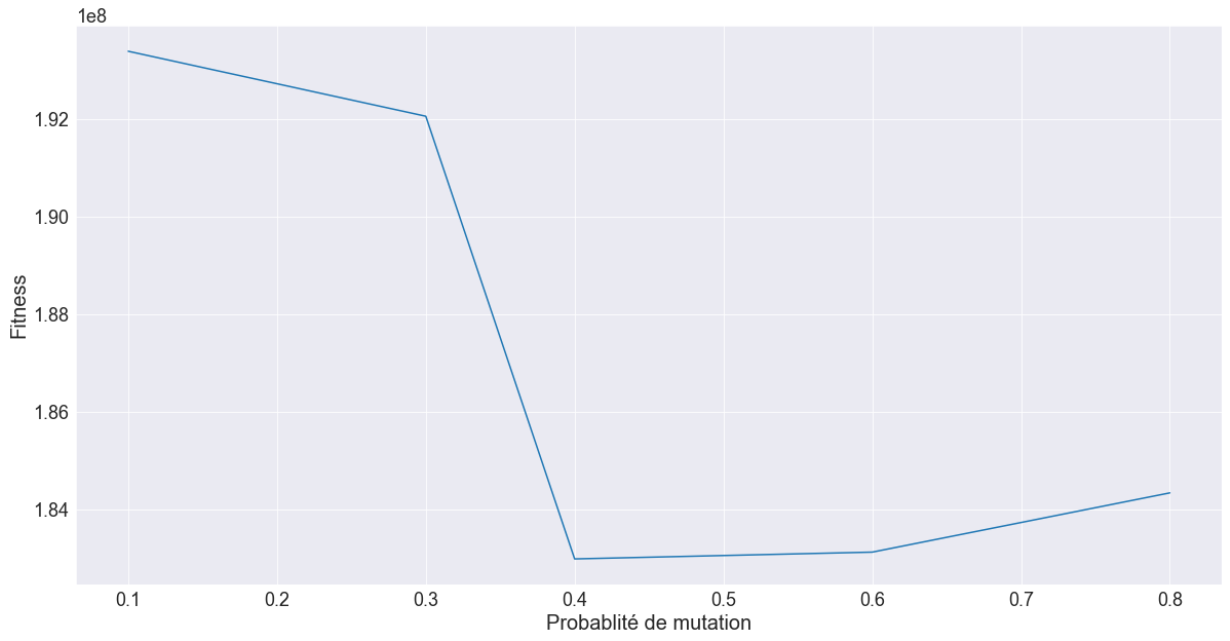
\includegraphics[keepaspectratio = true,scale=0.65]{mutation_mean.png}
\end{figure}
% back cover
\imtaMakeCover

\end{document}
%%%%%%%%%% END %%%%%%%%%% 
%%%%%%%%%%%%%%%%%%%%%%%%% 
